\documentclass[9pt]{beamer}
\setbeamertemplate{bibliography item}[text]
\mode<presentation> { \usetheme{Rochester} }
\usepackage{graphicx}

\title[Forest Fire Detection Review Report]
{Forest Fire Detection Review Report}

% \subtitle{3 literature reviews report}
\author[Author, Shun Li] {Shun Li\inst{1}}
\institute[Concordia]{Concordia University}
\date {\today}

% begin the slides
\begin{document}

\frame{\titlepage}
\begin{frame}
    \frametitle{Table of Contents}
    \tableofcontents
\end{frame}

\section{A review of machine learning applications in wildfire science and
management}

%1
\begin{frame}
    \frametitle{\textit{A review of machine learning applications in wildfire
    science and management} ~~------~~ Overview}
    \begin{columns}[t]
        \column{0.45\textwidth}
        \begin{block}{Applications}
            The application on the wild fire can be sperated into 6 domians
            (the problem domain):
        \end{block}
        \begin{itemize}
            \item fuels characterization, \textbf{fire detection and mapping}
            \item fire weather and climate change
            \item fire occurrence and risk
            \item \textbf{fire behavior prediction}
            \item fire effects
            \item \textbf{fire management}
        \end{itemize}

        \column{0.45\textwidth}
        \begin{block}{ML Methods}
            The most often used ML model across all of the problem domains:
        \end{block}
        \begin{itemize}
            \item Traditional Methods:
                \begin{itemize}
                    \item random forest (RF)
                    \item[*] maximum entropy (MaxEnt)\footnotemark[1]
                    \item artificial neural network (ANN)
                    \item decision tree (DT)
                    \item support vector machine (SVM)
                    \item genetic algorithm (GA)
                \end{itemize}
            \item Modern Methods:
                \begin{itemize}
                    \item deep learning (including the CNN, LSTM and other object
                        detection methods)
                    \item agent-based learning (including the Renforcement
                        Learning)
                \end{itemize}
        \end{itemize}
    \end{columns}
    \footnotetext[1]{The item with * should be studied later if needed.}
\end{frame}

%2
\begin{frame}
    \frametitle{\textit{A review of machine learning applications in wildfire
    science and management} ~~------~~ Main Tasks}
    \begin{enumerate} 
        \item fuels characterization, \textbf{fire detection and mapping:}\\
            \begin{itemize}
                \item \textbf{Detection (Classification + Regression problem
                    $\rightarrow$ Object Detection):}

                    Automatically detecting the wildfires as soon as possible,
                    even it is realtively small, with heat signatures or smoke
                    in infra-red or optical images, which can extend  spatial
                    and temporal coverage of the detection.

                \item \textbf{Mapping (Classification):} 
                    Classify the burned and unburned area to get the perimeter
            \end{itemize}
        \item \textbf{fire behavior prediction (Regression )\footnotemark[1]}:

            The papers in this area mainly deal with the larger scale processes
            and characteristics to predict or estimate the fire spread rates,
            fire growth, burned area, and fire severity.

        \item \textbf{fire management (Optimization, Regression)}:

            To have the appropriate amount of fire on the land.
            \begin{itemize}
                \item Optimize the allocation of the people, watchtower or other
                    fire-managing elements.
                \item Estimate the relationship of the fire characteristics and
                    the wild fire responds and even the social factors.
            \end{itemize}
    \end{enumerate}
    \colorbox{orange}{However, may be we can do more further about these
    applications!}
    \footnotetext[1]{not sure.}

\end{frame}

%3
\begin{frame}
    \frametitle{\textit{A review of machine learning applications in wildfire
    science and management} ~~------~~ Proposed Theories and Methods}

    The input data could be images, infra-images, multispectral images and MOIDS
    hotpot data from the UAVs, manned aircraft, watchtower, and satellite
    \begin{table}[H]
        \centering
        \begin{tabular}{p{0.3\textwidth}p{0.3\textwidth}p{0.3\textwidth}}
            \hline
            \textbf{Application Type} & Traditional Methods                    & Modern Methods  \\
            \hline
            fire detection            & ANN+infra SVM+video GA+LiDAR ANFIS     & CNN LSTM YOLO Optica-Flow 3D-CNN    \\
            fire mapping              & RF ANN SVM GPR(GP regression) AdaBoost & DNN    \\
            fire behavior prediction  & RF BNs KNN GA+physical model MDP       & CNN LSTM    \\
            fire management           & GA(optimization) BN ANN                & $\backslash$\\
            \hline
        \end{tabular}
        \caption{proposed methods}
    \end{table}
    \begin{itemize}
        \item \textbf{Traditional Methods:} Usually extract the images' feature
            with the computer vision technology, for example, the
            color(may under differernt color sapce) , texture,
            feature descriptors, etc.
        \item \textbf{Modern Methods:} usually the end-to-end model, use the
            convolution layers to `extract features`, the features are
            usually incomprehensible.
    \item \textbf{Mixed Methods:} Fast-RCNN, Faster-RCNN+feature selecting based on
            fuzzy logic
    \end{itemize}

\end{frame}

\section{A Review on Early Forest Fire Detection Systems
Using Optical Remote Sensing}

%1
\begin{frame}
    \frametitle{\textit{A Review on Early Forest Fire Detection Systems
Using Optical Remote Sensing ~------~ Overview}}

    There are 3 levels of the smoke and early fire detection system according to
    this review.
    \begin{itemize}
        \item System(platform)
        \item Sensors(types)
        \item Methods(traditional + deep learning based)
    \end{itemize}
    \begin{figure}[H]
        \centering
        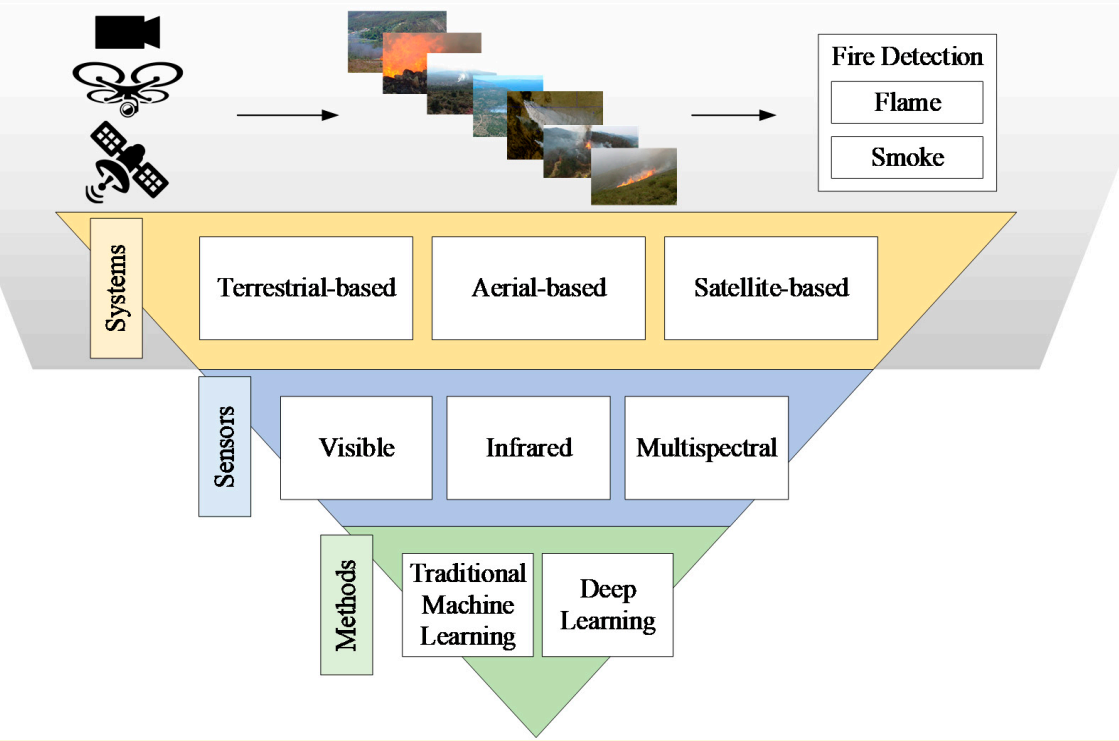
\includegraphics[width=0.6\textwidth]{./imgs/levels}
        \caption{the 3 levels of the detection systems}
    \end{figure}

\end{frame}

%2
\begin{frame}
    \frametitle{\textit{A Review on Early Forest Fire Detection Systems
Using Optical Remote Sensing ~------~ UAV based detection}}

UAVs can provide border and more accurate perception, get through a dangerous
and inaccessible zones.

\begin{columns}[t]
    \column{0.45\textwidth}
    \begin{block}{Traditional}
        \begin{itemize}
            \item noise reducing + color space + threshold = fire segmentation
            \item color space + Kalman filter = smoke detection
            \item color + motion features = fire and smoke segmentation(The
                flame has turbulent features $\rightarrow$ optical flow)
            \item (ROS + SLAM + DJIF550 = navigation) + (color, movement,
                temporal variation of fire intensity) = Simulation implementation
        \end{itemize}
    \end{block}

    \column{0.45\textwidth}
    \begin{block}{Deep learning based}
        \begin{itemize}
            \item Deep convolutional network(15 layers)
            \item Subregion selecting + YOLOv3 backbone + ZenMuse(4k) =
                detection
            \item YOLOv3(on ground station) + UAVs capturing $\rightarrow$ UAV
                flight path planning and replanning.
            \item fog computing + CNN = reducing the false alarm rate.
            \item 360-degree CMOS + DNN + fire dynamic texture = reduce the
                false alarm caused by the sunlight reflection and
                cloud.\footnotemark[1]

        \end{itemize}
    \end{block}

\end{columns}
\footnotetext[1]{The following paper}
\end{frame}

\section{Early Fire Detection Based on Aerial 360-Degree Sensors,
Deep Convolution Neural Networks and Exploitation of Fire Dynamic Textures}

%1
\begin{frame}
    \frametitle{\textit{Early Fire Detection Based on Aerial 360-Degree Sensors,
    Deep Convolution Neural Networks and Exploitation of Fire Dynamic Textures}}

    \Large 
    A multi-stages objection detection method is proposed, using:
    \normalsize
    \begin{itemize}
        \item \textbf{360-degree unlimited view image}
        \item \textbf{a novel post-validation adaptive method }
        \item \textbf{DeepLab V3+ model}
    \end{itemize}

    \begin{figure}[H]
        \centering
        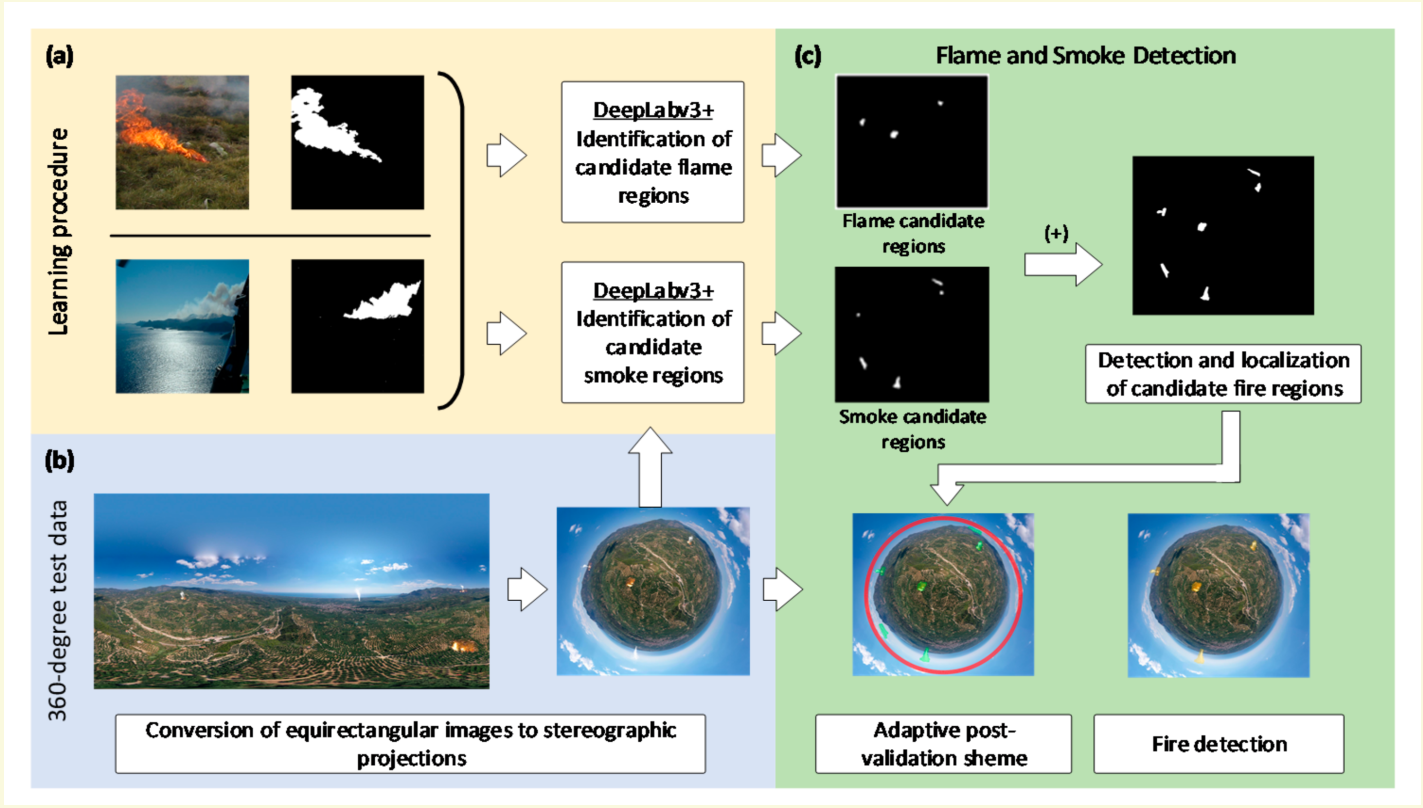
\includegraphics[width=0.7\textwidth]{./imgs/proposed_process}
    \end{figure}

\end{frame}

%2
\begin{frame}
    \frametitle{\textit{Early Fire Detection Based on Aerial 360-Degree Sensors
    ...  ~------~ Highlights}}

    \begin{itemize}
        \item \Large \colorbox{orange}{The 360-degree image:}\linebreak
            \normalsize
            Omnidirectional cameras can cover a wider field with only a single
            camera. Use the stereographic projection to map 3D to 2D.
        \item \Large \colorbox{orange}{The adaptive post-validation:}\linebreak
            \normalsize
            Use the KNN to cluster the cloud and the smoke around the horizon.
    \end{itemize}

    \begin{figure}[H]
        \centering
        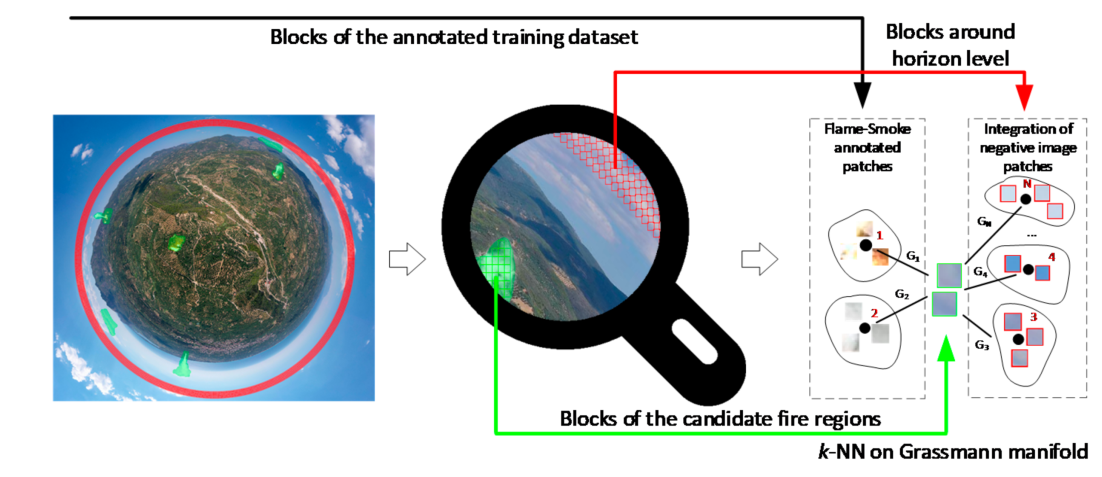
\includegraphics[width=0.7\textwidth]{./imgs/adaptive_validation}
    \end{figure}

\end{frame}

\section{The DJI M300 platform development }

\begin{frame}
    \frametitle{\textit{The DJI M300 platform development }
    ~~------~~ System Overview}
    \begin{figure}[H]
        \centering
        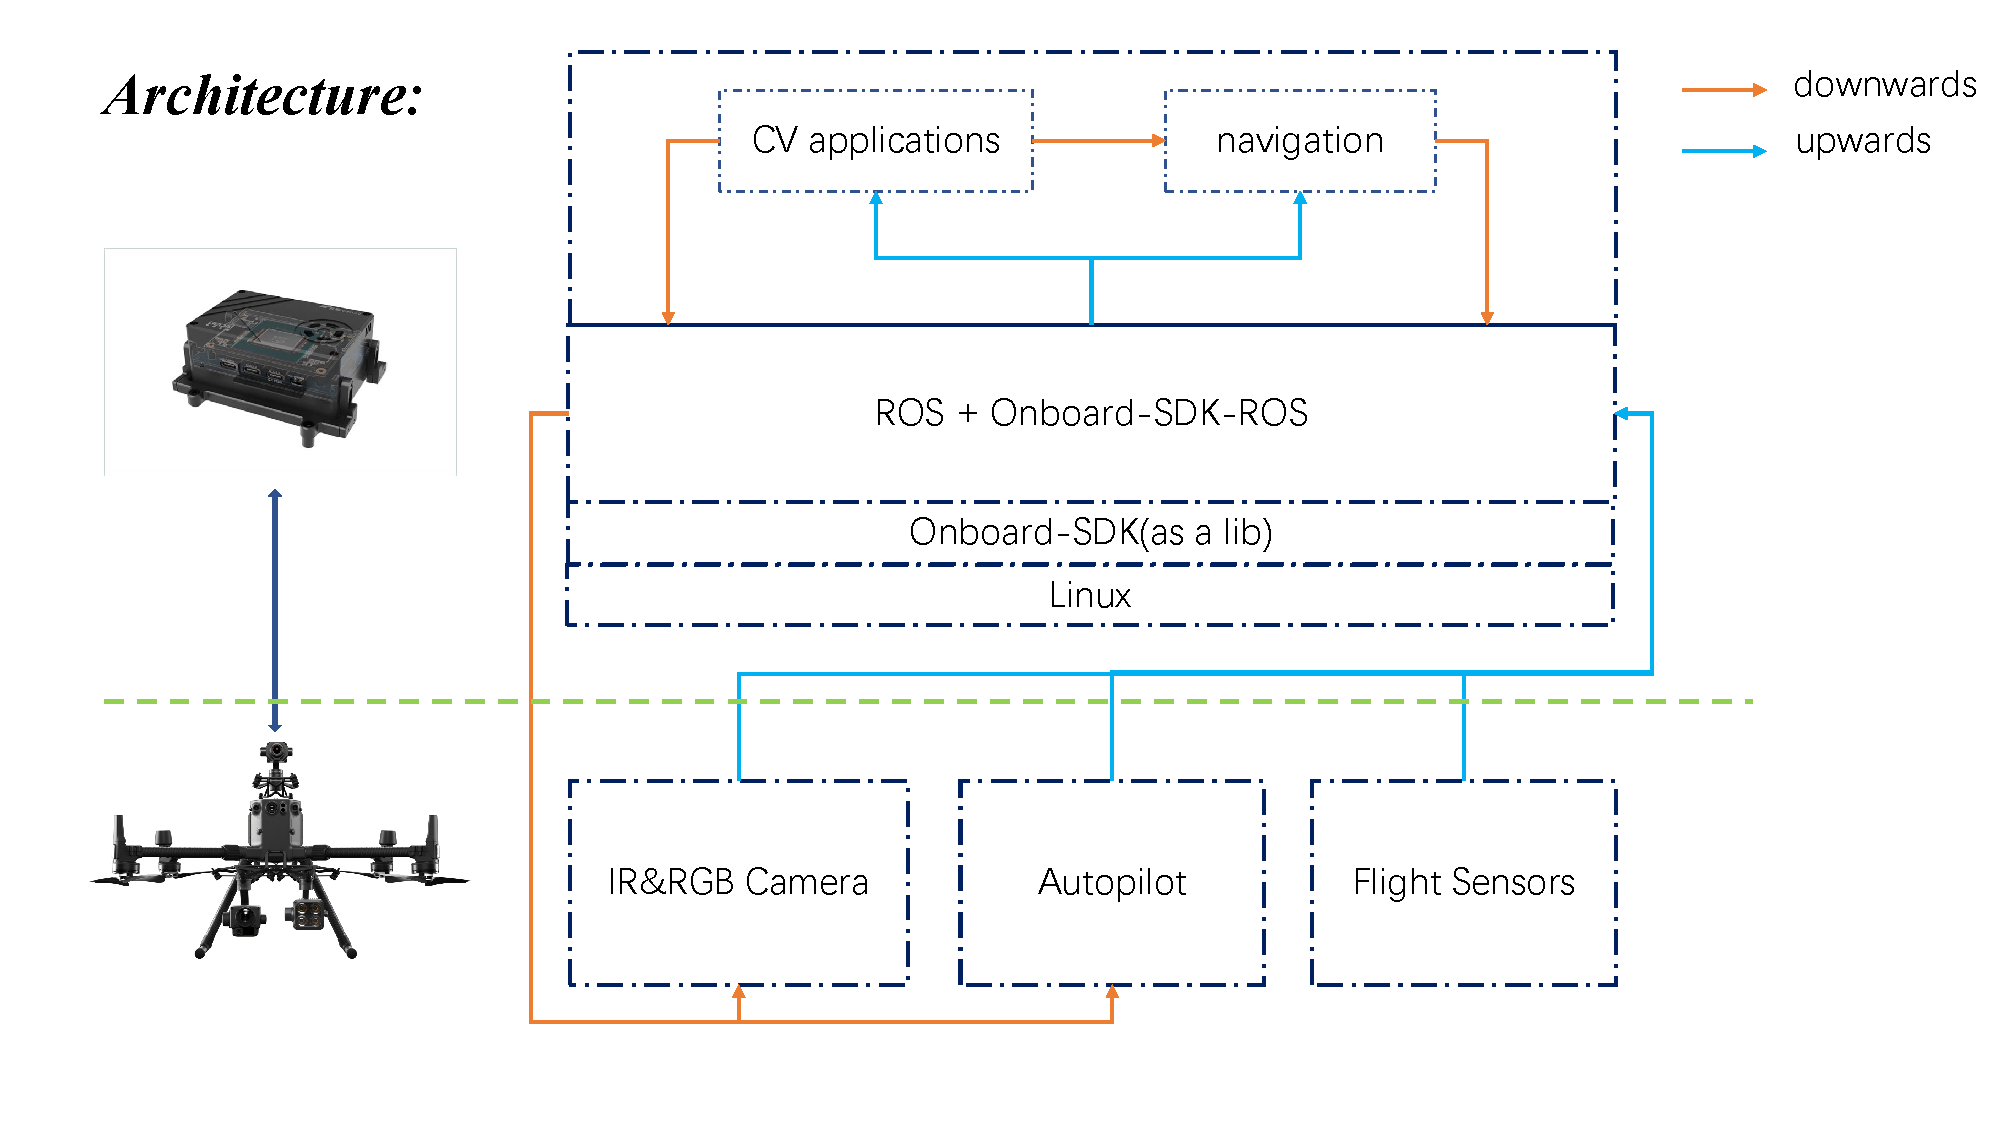
\includegraphics[width=1\textwidth]{./imgs/discuss.pdf}
    \end{figure}

    \colorbox{magenta}{Tasks:}
\begin{itemize}
    \item Computer Vision module for the fire and smoke detection.
    \item Navigation module for guidance.
\end{itemize}

\end{frame}

\section{Conclusion and Ideas:}
\begin{frame}
    \frametitle{Conclusion and Ideas:}

    \colorbox{orange}{\Large Conclusions:}
    \normalsize
    \begin{itemize}
        \item Some of the detection algorithms are ready to implemented on the
            drones.
        \item YOLO trends to have the lower accuracy to detect the small and
            overlap of the object comparing with RCNN, while the RCNN runs much
            slower than YOLO.
        \item The software environment and the communication of the M300 and
            YunGuan2 are tested in the past 1 week.
    \end{itemize}
    \colorbox{orange}{\Large Ideas:}
    \normalsize
    \begin{itemize}
        \item The next step to implement the aforementioned methods, and use the
            metrics to reproduce the basic algorithm as well as their derivates:
            \linebreak
            \begin{itemize}
                \item Implement the YOLO and some simple navigation algorithm on
                    the M300.
                \item Change the detection with Linhan's algorithm.
                \item Prepare for the flight test.
            \end{itemize}
    \end{itemize}
\end{frame}


% Insert a thank your frame 
\begin{frame}
    \Huge{\centerline{Thank you!}}
\end{frame}


\end{document}
